\documentclass[notes,11pt, aspectratio=169]{beamer}

\usepackage{pgfpages}
% These slides also contain speaker notes. You can print just the slides,
% just the notes, or both, depending on the setting below. Comment out the want
% you want.
\setbeameroption{hide notes} % Only slide
%\setbeameroption{show only notes} % Only notes
%\setbeameroption{show notes on second screen=right} % Both

\usepackage{helvet}
\usepackage[default]{lato}
\usepackage{array}
\usepackage{tgbonum}

\usepackage{tikz}
\usepackage{verbatim}
\setbeamertemplate{note page}{\pagecolor{yellow!5}\insertnote}
\usetikzlibrary{positioning}
\usetikzlibrary{snakes}
\usetikzlibrary{calc}
\usetikzlibrary{arrows}
\usetikzlibrary{decorations.markings}
\usetikzlibrary{shapes.misc}
\usetikzlibrary{matrix,shapes,arrows,fit,tikzmark}
\usepackage{amsmath}
\usepackage{mathpazo}
\usepackage{hyperref}
\usepackage{lipsum}
\usepackage{multimedia}
\usepackage{graphicx}
\usepackage{multirow}
\usepackage{graphicx}
\usepackage{dcolumn}
\usepackage{bbm}
\newcolumntype{d}[0]{D{.}{.}{5}}

\usepackage{changepage}
\usepackage{appendixnumberbeamer}
\newcommand{\beginbackup}{
   \newcounter{framenumbervorappendix}
   \setcounter{framenumbervorappendix}{\value{framenumber}}
   \setbeamertemplate{footline}
   {
     \leavevmode%
     \hline
     box{%
       \begin{beamercolorbox}[wd=\paperwidth,ht=2.25ex,dp=1ex,right]{footlinecolor}%
%         \insertframenumber  \hspace*{2ex} 
       \end{beamercolorbox}}%
     \vskip0pt%
   }
 }
\newcommand{\backupend}{
   \addtocounter{framenumbervorappendix}{-\value{framenumber}}
   \addtocounter{framenumber}{\value{framenumbervorappendix}} 
}


\usepackage{graphicx}
\usepackage[space]{grffile}
\usepackage{booktabs}
\newcommand\independent{\protect\mathpalette{\protect\independenT}{\perp}}
\def\independenT#1#2{\mathrel{\rlap{$#1#2$}\mkern2mu{#1#2}}}
\DeclareMathOperator{\Supp}{Supp}

% These are my colors -- there are many like them, but these ones are mine.
\definecolor{blue}{RGB}{0,114,178}
\definecolor{red}{RGB}{213,94,0}
\definecolor{yellow}{RGB}{240,228,66}
\definecolor{green}{RGB}{0,158,115}

\hypersetup{
  colorlinks=false,
  linkbordercolor = {white},
  linkcolor = {blue}
}


%% I use a beige off white for my background
\definecolor{MyBackground}{RGB}{255,253,218}

%% Uncomment this if you want to change the background color to something else
%\setbeamercolor{background canvas}{bg=MyBackground}

%% Change the bg color to adjust your transition slide background color!
\newenvironment{transitionframe}{
  \setbeamercolor{background canvas}{bg=yellow}
  \begin{frame}}{
    \end{frame}
}

\setbeamercolor{frametitle}{fg=blue}
\setbeamercolor{title}{fg=black}
\setbeamertemplate{footline}[frame number]
\setbeamertemplate{navigation symbols}{} 
\setbeamertemplate{itemize items}{-}
\setbeamercolor{itemize item}{fg=blue}
\setbeamercolor{itemize subitem}{fg=blue}
\setbeamercolor{enumerate item}{fg=blue}
\setbeamercolor{enumerate subitem}{fg=blue}
\setbeamercolor{button}{bg=MyBackground,fg=blue,}



% If you like road maps, rather than having clutter at the top, have a roadmap show up at the end of each section 
% (and after your introduction)
% Uncomment this is if you want the roadmap!
% \AtBeginSection[]
% {
%    \begin{frame}
%        \frametitle{Roadmap of Talk}
%        \tableofcontents[currentsection]
%    \end{frame}
% }
\setbeamercolor{section in toc}{fg=blue}
\setbeamercolor{subsection in toc}{fg=red}
\setbeamersize{text margin left=1em,text margin right=1em} 

\newenvironment{wideitemize}{\itemize\addtolength{\itemsep}{10pt}}{\enditemize}

\usepackage{environ}
\NewEnviron{videoframe}[1]{
  \begin{frame}
    \vspace{-8pt}
    \begin{columns}[onlytextwidth, T] % align columns
      \begin{column}{.70\textwidth}
        \begin{minipage}[t][\textheight][t]
          {\dimexpr\textwidth}
          \vspace{8pt}
          \hspace{4pt} {\Large \sc \textcolor{blue}{#1}}
          \vspace{8pt}
          
          \BODY
        \end{minipage}
      \end{column}%
      \hfill%
      \begin{column}{.38\textwidth}
        \colorbox{green!20}{\begin{minipage}[t][1.2\textheight][t]
            {\dimexpr\textwidth}
            Face goes here
          \end{minipage}}
      \end{column}%
    \end{columns}
  \end{frame}
}

\title[]{\textcolor{blue}{Canonical Research Designs III:\\ Instrumental Variables I }}
\author[PGP]{}
\institute[FRBNY]{\small{\begin{tabular}{c}
  Paul Goldsmith-Pinkham  \\
\end{tabular}}}

\date{\today}

\begin{document}

%%% TIKZ STUFF
\tikzset{   
        every picture/.style={remember picture,baseline},
        every node/.style={anchor=base,align=center,outer sep=1.5pt},
        every path/.style={thick},
        }
\newcommand\marktopleft[1]{%
    \tikz[overlay,remember picture] 
        \node (marker-#1-a) at (-.3em,.3em) {};%
}
\newcommand\markbottomright[2]{%
    \tikz[overlay,remember picture] 
        \node (marker-#1-b) at (0em,0em) {};%
}
\tikzstyle{every picture}+=[remember picture] 
\tikzstyle{mybox} =[draw=black, very thick, rectangle, inner sep=10pt, inner ysep=20pt]
\tikzstyle{fancytitle} =[draw=black,fill=red, text=white]
%%%% END TIKZ STUFF

% Title Slide
\begin{frame}
\maketitle
\end{frame}


\begin{frame}{Today's topic}
  \begin{wideitemize}
  \item In many examples, we've worried about estimating the effect
    of some treatment $D_{i}$ on $Y_{i}$, but concerned that this
    estimate will be biased
  \item In circumstances where we had strong ignorability (due to
    perhaps randomization), we felt confident that this was not a concern
  \item But what about when this isn't the case?
  \begin{itemize}
    \item  We need to \emph{create}  ``as-if'' random variation in $D_{i}$
  \end{itemize}
  \item The very popular solution: instrumental variables
  \end{wideitemize}
\end{frame}

\begin{frame}{Today's topic}
  \begin{wideitemize}
  \item There is a huge amount of material to cover regarding IV
  \item Today, we will be covering the setup and overview for how to think about IV
  \item Next class, covering a wide range of practical issues and
    problems that come up for researchers working on these topics
  \end{wideitemize}
\end{frame}

\begin{frame}{Many faces of Instrumental Variables}
  \begin{wideitemize}
  \item  This class is clearly not the first place you've been exposed to IV
    \begin{itemize}
    \item Now so ubiqutous that likely seen multiple times
    \end{itemize}
  \item More interestingly, you've likely seen it in many forms
  \item To start class, we'll discuss what an IV approach can mean or
    looks like in the three types of tools we discussed way back in
    Lecture 1
    \begin{enumerate}
  \item First, we'll try to define what we mean by an instrumental
    variable, initially using the DAG notation
  \item Then, we'll discuss the classic structural econometrics
    modeling form, and link it to GMM
    \begin{itemize}
    \item Moments!
    \end{itemize}
  \item Finally, we'll discuss the potential outcomes or design-based
    setup
    \end{enumerate}
  \end{wideitemize}
\end{frame}

\begin{frame}{What is an instrumental variable?}
  \only<1>{  \includegraphics[width=\linewidth]{images/angristiva.png}}
  \only<2>{  \includegraphics[width=\linewidth]{images/angristivb.png}}
  \only<3>{  \includegraphics[width=\linewidth]{images/angristivc.png}
    \includegraphics[width=\linewidth]{images/angristivd.png}}  
\end{frame}

\begin{frame}{What is an instrumental variable?}
  \includegraphics[width=\linewidth]{images/mheiva.png}
\begin{wideitemize}
  \item Variables that do the shifting!
\end{wideitemize}
\end{frame}

\begin{frame}{The curve shifting example}
  \begin{wideitemize}
  \item Consider a simple supply and demand curve setup
    \begin{align}
      \text{quantity}_{d} &= \alpha_{1} + \text{price}\gamma_{1} + W_{1}\tau_{1} + u_{1}\\
      \text{quantity}_{s} &= \alpha_{2} + \text{price}\gamma_{2} + W_{2}\tau_{2} + u_{2}
    \end{align}
  \item Equilibrium values of price and quantity are such that these
    equations equal
    \begin{itemize}
    \item These can vary due to many various regions -- they can be
      specific to demand or supply, or happen to both
    \end{itemize}
  \item The \emph{observed} values of price and quantity will give a
    cloud of points with no real interpretation as either demand or
    supply curve coefficients (elasticities)

  \item What we need is shifters of these curves to create variation
    that traces out either supply or demand
    \begin{itemize}
    \item Notably, this traces out only a local part of the curve!
    \end{itemize}
  \end{wideitemize}
  
\end{frame}

\begin{frame}{What is an instrumental variable?}
  \begin{columns}[T] % align columns
    \begin{column}{0.6\textwidth}
  \begin{wideitemize}
  \item ``Curve-shifting variable'' is not a particularly extensible concept
  \item Let's start with the definition in the context of a DAG
  \item Consider an effect we are interested in identifying: $D$ on $Y$
    \begin{itemize}
    \item In this setting, we know it is not identifiable
    \end{itemize}
  \end{wideitemize}
\end{column}
\begin{column}{0.4\textwidth}
  \begin{center}
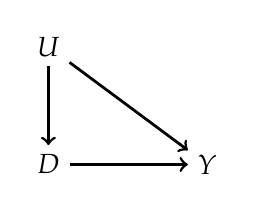
\begin{tikzpicture}
        % nodes %
        % \node[text centered] (z) {$Z$};
        \node[text centered] (t) {$D$};
        \node[right=1.5 of t, text centered] (y) {$Y$};
        \node[above = 1 of t, text centered] (u) {$U$};
        % \node[left = 1 of t, text centered] (z) {$Z$};        
        % edges %
        % \draw[->, line width= 1] (z) --  (t);
        \draw [->, line width= 1] (t) -- (y);
        % \draw[->,red, line width= 1,dashed] (u) --node {X} (z);
        \draw[->,line width= 1] (u) --(t);
%        \draw[->,line width= 1] (z) --(t);
 %       \draw[->,bend right, line width= 1] (z) to [out=-50,in=-130]  (y);                
        \draw[->,line width= 1] (u) -- (y);
%\draw[->, red, line width=1,dashed] (z) to  [out=270,in=270, looseness=0.5] node{X} (y);
      \end{tikzpicture}
      \end{center}
\end{column}
\end{columns}
\end{frame}

\begin{frame}{What is an instrumental variable?}
  \begin{columns}[T] % align columns
    \begin{column}{0.6\textwidth}
      \begin{wideitemize}
      \item Now, we have a variable $Z$ which can identify two effects:
        \begin{itemize}
        \item $Z$ on $D$
        \item $Z$ on $Y$
        \end{itemize}
      \item What is the content of this instrumental variable, $Z$?
        \begin{itemize}
        \item It  affects $Y$ (\textbf{Relevance})                    
        \item It only affects $Y$ through $D$ (\textbf{Exclusion})
        \end{itemize}
      \item Without further assumptions, it won't be possible to
        identify the effect of $D$ on $Y$ using this, but it
        highlights the features of an IV
        \begin{itemize}
        \item We'll discuss why shortly
        \end{itemize}
      \end{wideitemize}
\end{column}
\begin{column}{0.4\textwidth}
  \begin{center}
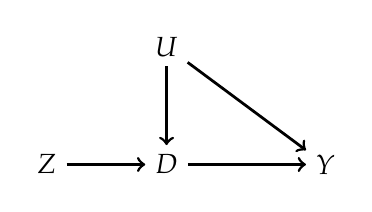
\begin{tikzpicture}
        % nodes %
        % \node[text centered] (z) {$Z$};
        \node[text centered] (t) {$D$};
        \node[right=1.5 of t, text centered] (y) {$Y$};
        \node[above = 1 of t, text centered] (u) {$U$};
         \node[left = 1 of t, text centered] (z) {$Z$};        
        % edges %
        % \draw[->, line width= 1] (z) --  (t);
        \draw [->, line width= 1] (t) -- (y);
        % \draw[->,red, line width= 1,dashed] (u) --node {X} (z);
        \draw[->,line width= 1] (u) --(t);
        \draw[->,line width= 1] (z) --(t);
 %       \draw[->,bend right, line width= 1] (z) to [out=-50,in=-130]  (y);                
        \draw[->,line width= 1] (u) -- (y);
%\draw[->, red, line width=1,dashed] (z) to  [out=270,in=270, looseness=0.5] node{X} (y);
      \end{tikzpicture}
      \end{center}
\end{column}
\end{columns}
\end{frame}

\begin{frame}{Structural version of instruments - GMM and 2SLS}
  \begin{wideitemize}
  \item The canonical setup with an IV:
    \begin{align*}
      Y_{i} &= D_{i}\beta + W_{i}\gamma_{1} + \epsilon_{i}\\
      D_{i} &= Z_{i}\pi + W_{i}\gamma_{2} + u_{i}
    \end{align*}
    with $W_{i}$ are a set of exogeneous controls
  \item A couple notable features about this setup:
    \begin{itemize}
    \item We've assumed a very parametric model for $Y_{i}$
    \item In particular, we've assumed a constant effect of $D_{i}$ on $Y_{i}$
    \end{itemize}
  \item The necessary assumptions to identify $D_{i}$ in this setting are straightforward:
    \begin{itemize}
    \item Relevance: $\pi \not = 0$
    \item Exclusion: $E(\epsilon_{i}Z_{i} | W_{i}) = 0$
    \end{itemize}
  \end{wideitemize}
\end{frame}

\begin{frame}{Structural version of instruments - GMM and 2SLS}
  \begin{wideitemize}
  \item The exclusion restriction can be slightly opaque
    \begin{itemize}
    \item The $\epsilon_{i}$ captures the set of ``other'' things that can happen
    \item But can be harder to map into a counterfactual way of discussing outcomes
    \end{itemize}
  \item One useful result: let $Z_{i}^{*} = Z_{i} - E(Z_{i} | W_{i})$
    \begin{itemize}
    \item Then the exclusion restriction can be viewed as saying that
      $E(\epsilon_{i}Z_{i}^{*}) = 0$
    \item That is, the variation in $Z_{i}$ above and beyond $W_{i}$
      has to be exogeneous for $\epsilon_{i}$
    \end{itemize}
  \item Why is this often written as a system of linear equations?
    \begin{itemize}
    \item Historical precedent is part of it -- linear demand systems
    \item But, it turns out it is ``optimal'' in a particular sense
    \end{itemize}
  \end{wideitemize}
\end{frame}

\begin{frame}{Structural version of instruments - GMM and 2SLS}
  \begin{wideitemize}
  \item   In GMM, there's just a more general statement -- ignore the first stage for a moment
    \begin{itemize}
    \item We still maintain the linear second stage -- the
      ``structural model''
    \item To write this compactly, let $\widetilde{D}_{i} = (D_{i}, W_{i})$ and $\widetilde{Z}_{i} = (Z_{i}, W_{i})$
    \end{itemize}
  \item Recall that the exclusion restriction gives us a set of $K$ \emph{moments}. 
    \begin{itemize}
    \item $E((Y_{i} - D_{i}\beta - W_{i}\gamma)Z_{i})$ (excluded instruments)
    \item $E((Y_{i} - D_{i}\beta - W_{i}\gamma)W_{i})$ (exogeneous instruments)
    \item Or compactly,
      $\mathbf{g}(\beta, \gamma) = E((Y_{i} -
      \widetilde{D}_{i}\widetilde{\beta})\widetilde{Z}_{i})$
    \end{itemize}
  \item Then, recall that given these $K$ moments, for a $K \times K$
    positive-definite weight matrix $\Omega$, we can define our linear GMM
    estimator as the solution to the following problem:
    \begin{align}
      (\beta_{0}, \gamma_{0}) &= \arg\min_{\beta, \gamma} \mathbf{g}(\beta, \gamma)' \Omega \mathbf{g}(\beta, \gamma)
    \end{align}
  \end{wideitemize}
\end{frame}

\begin{frame}{Structural version of instruments - GMM and 2SLS}
  \begin{wideitemize}
  \item Fortunately, because $\mathbf{g}$ is linear, solving for the minimizer is analytically tractable
    \begin{itemize}
    \item More non-linear second stages are solveable as well, but typically need numerical solutions
    \end{itemize}
  \item Our general solution is a function of our choice of $\Omega$:
    \begin{align*}
      \hat{\widetilde{\beta}} = \frac{\widetilde{D}'\widetilde{Z} \Omega \widetilde{Z}'\widetilde{Y}}{\widetilde{D}'\widetilde{Z} \Omega \widetilde{Z}'\widetilde{D}}
    \end{align*}
  \item Turns out that if the exclusion restriction holds (and
    relevance, such that the denominator isn't zero), it really
    doesn't matter what $\Omega$ is -- your estimator will converge
    \begin{itemize}
    \item If there's no unobserved heterogeneity in $\beta$!
    \begin{equation*}
      \hat{\widetilde{\beta}} -\widetilde{\beta} = \frac{\widetilde{D}'\widetilde{Z} \Omega \widetilde{Z}'\epsilon}{\widetilde{D}'\widetilde{Z} \Omega \widetilde{Z}'\widetilde{D}} \rightarrow 0
    \end{equation*}
    \item All thanks to $E(\widetilde{Z}\epsilon) = 0$
    \end{itemize}
  \end{wideitemize}
\end{frame}

\begin{frame}{Structural version of instruments - GMM and 2SLS}
  \begin{wideitemize}
  \item Where does 2SLS come in? Contrast the formula for 2SLS and this GMM estimator:
    \begin{align*}
      \hat{\widetilde{\beta}}_{2SLS} &= \frac{\widetilde{D}'\widetilde{Z} (\widetilde{Z}'\widetilde{Z})^{-1} \widetilde{Z}'\widetilde{Y}}{\widetilde{D}'\widetilde{Z} (\widetilde{Z}'\widetilde{Z})^{-1} \widetilde{Z}'\widetilde{D}}\\ 
      \hat{\widetilde{\beta}}_{GMM} &= \frac{\widetilde{D}'\widetilde{Z} \Omega \widetilde{Z}'\widetilde{Y}}{\widetilde{D}'\widetilde{Z} \Omega \widetilde{Z}'\widetilde{D}}
    \end{align*}
  \item 2SLS is a special GMM setting with the weight matrix equal to
    the inverse of the covariance of the instruments
    \begin{itemize}
    \item Recall that in GMM, there are ways to get ``better'' weight
      matrices to minimize the variance of the estimator (e.g. 2-step
      GMM, iterated GMM, etc.)
    \item However, it turns out 2SLS weight matrix is optimal under
      homoskedasticity!
    \end{itemize}
  \end{wideitemize}
\end{frame}


\begin{frame}{Some useful features of 2SLS}
    \begin{align*}
      \hat{\widetilde{\beta}}_{2SLS} &= \frac{\widetilde{D}'\widetilde{Z} (\widetilde{Z}'\widetilde{Z})^{-1} \widetilde{Z}'\widetilde{Y}}{\widetilde{D}'\widetilde{Z} (\widetilde{Z}'\widetilde{Z})^{-1} \widetilde{Z}'\widetilde{D}}
    \end{align*}
  \begin{wideitemize}
  \item Recall the projection matrix
    $P_{Z} = \widetilde{Z} (\widetilde{Z}'\widetilde{Z})^{-1}
    \widetilde{Z}'$
    \begin{itemize}
    \item Important property: idempotency -- e.g. $P_{Z}P_{Z} = P_{Z}$
    \end{itemize}
    \begin{align*}
      \hat{\widetilde{\beta}}_{2SLS} &= \frac{\widetilde{D}'P_{Z}P_{Z}\widetilde{Y}}{\widetilde{D}'P_{Z}P_{Z}\widetilde{D}} = \frac{\hat{\widetilde{D}}'\hat{\widetilde{Y}}}{\hat{\widetilde{D}}'\hat{\widetilde{D}}} 
    \end{align*}
  \item Hence it's really the projection of $D$ onto $Z$, and the
    projection of $Y$ onto $Z$
    \begin{itemize}
    \item So the numerator is the covariance of the predicted pieces,
      and the denominator is the variance of the predicted endogeneous
      variable
    \end{itemize}
  \item This is exactly what our curve shifter had in mind -- we need
    variation in the predicted values
  \end{wideitemize}
\end{frame}

\begin{frame}{Structural version of instruments - GMM and 2SLS}
  \begin{wideitemize}
  \item This approach is focusing on a parameteric specification, but
    the important assumption is that $E(\epsilon_{i}Z_{i}) = 0$ and
    $E(D_{i}Z_{i}) \not=0$. Note that this is much weaker than random
    assignment!
  \item But, it is kind of wonky to assume mean independence and not
    assume full independence
  \item Why? Well, consider transforming the outcome $Y$ by taking a
    log (or some other nonlinear transformation). With only mean
    indpeendence, our instrument is not necessarily valid anymore.
    \begin{itemize}
    \item That seems like a undesirable property!
    \item Unfortunately, comparable to our discussion of difference-in-difference!
    \end{itemize}
  \end{wideitemize}
\end{frame}

\begin{frame}{The necessary assumptions so far}
  \begin{wideitemize}
  \item So far, we need the following assumptions (and this is what
    you should always discuss when writing a paper on IV):
    \begin{enumerate}
    \item   relevance $E(D_{i}Z_{i}) $
    \item exclusion $E(Z_{i}\epsilon_{i})$
    \end{enumerate}
  \item Tricky part starts now. Two issues with this setup:
    \begin{itemize}
    \item we have assumed homogeneous effects. E.g. $\beta$ is the
      same for all individuals.
      \begin{itemize}
      \item This is fixable in the model, but question is what
        estimand do we have?
      \end{itemize}
    \item It's not a very coherent ``design-based'' setup. In other
      words, it's challenging to think about the shifter $Z$ in terms
      of the potential outcomes of the outcomes
      \begin{itemize}
      \item This can make it hard to suss out the validity of the design!
      \end{itemize}
    \end{itemize}
  \item Large literature in the 1990s (and continuing forward) focused
    on taking the Neyman-Rubin Casual Model (NRCM) with potential
    outcomes and mapping it to IV
    \begin{itemize}
    \item Pushed by Josh Angrist, Guido Imbens, and Don Rubin
    \end{itemize}
  \end{wideitemize}
\end{frame}

\begin{frame}{Imbens and Angrist  (1994)}
  \begin{wideitemize}
  \item Start by focusing on the simplest of cases: binary instrument
    $Z$, binary treatment $D$, and no controls
  \item Potential outcomes framework needs to be extended to allow an instrument!
    \begin{itemize}
    \item Define $Y_{i}(D_{i}(Z_{i}), Z_{i})$ and $D_{i}(Z_{i})$ as two forms of potential outcomes
    \item The \emph{exclusion} restriction here is that
      $Y_{i}(D_{i}(Z_{i}), Z_{i}) =Y_{i}(D_{i}(Z_{i}))$, e.g. $Z_{i}$
      only has an effect on $Y_{i}$ through $D_{i}$
    \item \emph{Relevance} is that $P(w) = E(D_{i} | Z_{i} = w)$ varies across $w$
    \end{itemize}
  \item  Key point is the $Y_{i}(1) - Y_{i}(0)$ can be different for every individual
    \begin{itemize}
    \item Unlike in the structural models we wrote before, where $\beta$ was constant
    \end{itemize}
  \item We'll assume that $Z$ is completely randomly assigned relative
    to the potential outcomes of $Y$ and $D$
  \end{wideitemize}
\end{frame}

\begin{frame}{No ATE is guaranteed  - Imbens and Angrist  (1994)}
  \begin{wideitemize}
  \item Key point: consider $E(Y_{i} | Z_{i} = 1) - E(Y_{i} | Z_{i} = 0)$ (where $P(1) > P(0)$)
    \begin{align*}
      E(Y_{i} | Z_{i} = 1) - E(Y_{i} | Z_{i} = 0) &= E(D_{i}(1)Y_{i}(1) + (1-D_{i}(1))Y_{i}(0)  | Z_{i} = 1)\\
                                                  &- E(D_{i}(0)Y_{i}(1) + (1-D_{i}(0))Y_{i}(0)  | Z_{i} = 0)\\
                                                  &= E((D_{i}(1) - D_{i}(0))(Y_{i}(1) - Y_{i}(0)))\\
      = Pr(D_{i}(1) - D_{i}(0) = 1) \times &E(Y_{i}(1) - Y_{i}(0)) | D_{i}(1) - D_{i}(0) = 1) \\
      - Pr(D_{i}(1) - D_{i}(0) = -1) \times &E(Y_{i}(1) - Y_{i}(0)) | D_{i}(1) - D_{i}(0) = -1) \\
    \end{align*}
  \item There's a lot to unpack here.
  \end{wideitemize}
\end{frame}


\begin{frame}{No ATE is guaranteed  - Imbens and Angrist  (1994)}
    \begin{align*}
      E(Y_{i} | Z_{i} = 1) - E(Y_{i} | Z_{i} = 0) &= \\
      = Pr(D_{i}(1) - D_{i}(0) = 1) \times &E(Y_{i}(1) - Y_{i}(0)) | D_{i}(1) - D_{i}(0) = 1) \\
      - Pr(D_{i}(1) - D_{i}(0) = -1)& \times E(Y_{i}(1) - Y_{i}(0)) | D_{i}(1) - D_{i}(0) = -1) 
    \end{align*}
  \begin{wideitemize}
  \item First, note that while we assumed that the propensity score
    was increasing, it does \emph{not} imply that it's increasing for
    everyone
  \item Second, we are only identifying the effects of $D$
    ($Y_{i}(1) - Y_{i}(0)$) for those individuals who behavior shifted
    due to the change in $Z$
  \item Third, without restrictions on $Y_{i}$, this effect can be
    zero or even negative, even if the true causal effect is positive!
    \begin{itemize}
    \item Those shifted into participating by $Z$ could be exactly
      cancelled by those who shift out
    \end{itemize}
  \end{wideitemize}
\end{frame}

\begin{frame}{Local Average Treatment Effect (LATE)}
  \begin{wideitemize}
  \item Two potential solutions to this issue:
    \begin{enumerate}
      \item In a constant effects world, this problem does not exist!
      \item Secondly, if there exists an instrument such that
        $Pr(D_{i}(1) - D_{i}(0) = -1) = 0$, then you're fine as well
        (e.g. one sided compliance)
    \end{enumerate}
  \item Key innovation: with \emph{monotonicity}, can identify the
    Local Average Treatment Effect
  \item \textbf{Monotonicity}: $D_{i}(1) \geq D_{i}(0))$ for all $i$ (or vice versa)
    \begin{itemize}
    \item All effects must be monotone in the same direction
    \item This is fundamentally untestable! (also suffers from
      fundamental problem of causal inference)
    \end{itemize}
    \vspace{-5pt}
  \item Conditional on assuming monotonicity, then the Wald ratio estimates the LATE:
    \begin{align*}
      \tau_{LATE}   & = \frac{E(Y_{i} | Z_{i} = 1) -E(Y_{i} | Z_{i} = 0)}{E(D_{i} | Z_{i} = 1) -E(D_{i} | Z_{i} = 0)} \\
      &=\frac{Pr(D_{i}(1) - D_{i}(0) = 1) \times E(Y_{i}(1) - Y_{i}(0)) | D_{i}(1) - D_{i}(0) = 1)}{E(D_{i} | Z_{i} = 1) -E(D_{i} | Z_{i} = 0)} \\
      &=E(Y_{i}(1) - Y_{i}(0)) | D_{i}(1) - D_{i}(0) = 1)
    \end{align*}
  \end{wideitemize}
\end{frame}

\begin{frame}{What does this mean?}
  \begin{wideitemize}
  \item Fundamentally, this means that an IV strategy only identifies
    (non-parametrically) the effect of a treatment for those who
    respond to the treatment.
    \begin{itemize}
    \item     Monotonicity ensures that the responders all go in one direction
    \end{itemize}
  \item Language used to describe these groups:
    \begin{itemize}
    \item Always-takers: $D_{i}(1) = D_{i}(0) = 1$
    \item Never-takers: $D_{i}(1) = D_{i}(0) = 0$
    \item Compliers: $D_{i}(1) - D_{i}(0) = 1$
    \item Defiers: $D_{i}(1) - D_{i}(0) = -1$                   
    \end{itemize}
  \item Monotonicity ensures that only one of the compliers or defiers exists
    \begin{itemize}
    \item The compliers can be very different! This is a particular subgroup
    \item Important to understand potential differences
    \end{itemize}
  \end{wideitemize}
\end{frame}

\begin{frame}{Loosening restrictiveness + 2SLS}
  \begin{wideitemize}
  \item This setup is very specific (two binary measures) but it is
    straightforward to generalize to a multi-valued \emph{instrument}
  \item Slightly more challenging (notationally) to generalize to a multivalued
    treatment in a non-parametric way
    \begin{itemize}
    \item Key concept is an \textbf{average causal reponse curve} --
      effectively a combination of weighted derivatives, depending on
      where the instrument shifts participation
    \item  Angrist + Imbens (1995, JASA)
    \end{itemize}
  \end{wideitemize}
\end{frame}


\begin{frame}{Average Causal Response Curve}
  \begin{wideitemize}
  \item Consider a regression of (log) weekly earnings ($Y_{i}$) on
    years of schooling ($S_{i}$) with controls $W_{i}$, where we use
    the quarter-of-birth     ($Z_{i}$) to instrument for schooling
    \begin{equation*}
      Y_{i} = W_{i}\gamma + S_{i}\tau + \epsilon_{i}
    \end{equation*}
  \item Recall the potential outcome notation for years of schooling $\in \{0,\ldots, J\}$
    \begin{itemize}
    \item We can then consider relative comparisons: $\tau_{j,j-1} = E(Y_{i}(j) - Y_{i}(j-1))$
    \item Note that if this were a linear effect, $\tau_{j,j-1} = 0.5\tau_{j,j-2}$, etc.
    \end{itemize}
  \item Now consider the potential years of schooling defined by $Z_{i}$: $S_{i}(Z_{i})$
    \begin{itemize}
    \item Can consider this binary (first quarter vs. later)
    \end{itemize}
  \end{wideitemize}
\end{frame}

\begin{frame}{Average Causal Response Curve}
  \begin{wideitemize}
  \item Under independence assumptions and monotonicity
    ($S_{i}(1) -S_{i}(0) \geq 0$ or vice versa) for each person,
    \begin{equation*}
      \frac{E(Y_{i} | Z_{i} = 1) - E(Y_{i} | Z_{i} = 0)}{E(S_{i} | Z_{i} = 1) - E(S_{i} | Z_{i} = 0)} = \sum_{j=1}^{J}\omega_{j}E(Y_{i}(j) - Y_{i}(j-1) | S_{i}(1) \geq j > S_{i}(0))
    \end{equation*}
    where
    \begin{equation*}
      \omega_{j} = \frac{Pr(S_{i}(1) \geq j > S_{0})}{\sum_{i=1}^{J} Pr(S_{i}(1) \geq i > S_{0})}.
      \end{equation*}
    \item $\omega_{j}$ can be consistently estimated using the data
  \item Key takeaway: weighting up non-parametric treatments as a
    function of where the instrument induces response
  \end{wideitemize}
\end{frame}

\begin{frame}{Average Causal Response Curve weights}
 \includegraphics[width=0.8\linewidth]{images/angrist_imbens_acr_weight.png}
\end{frame}

\begin{frame}{Next class}
  \begin{wideitemize}
  \item   Monotonicity is a powerful tool for ensuring the weighted averages
    \begin{itemize}
    \item   but a remarkably strong assumption in some places!
    \end{itemize}
  \item If it fails, it doesn't mean that there isn't a causal effect
    identified, but researchers should be careful
    \begin{itemize}
    \item Next class, will discuss sensitivities and other issues
    \end{itemize}
  \item An important note: the IV estimate is just a rescaled reduced
    form estimate
    \begin{itemize}
    \item If $Z$ is truly randomly assigned, the reduced form is a valid estimate
      \item Do you inherently need the rescaled estimate? 
    \end{itemize}
  \end{wideitemize}
\end{frame}

\end{document}
